\chapter{Design}

Using the data gathered in the previous chapter, we design a product that can solve the requirements, listed at section \ref{Requirements}. In this chapter we split the product into modular components that contain its functionality and use this to design the program architecture. Afterwards, we define interfaces to be used for implementing the software of the product. Besides the software, we also decide upon the physical design of the car, including which sensors we will use. Lastly, we will plan how we are going to test whether the individual components of the car conform to the requirements or not.

\section{Components}

To start, we split the project into a number of smaller modular components, that, when put together, make up a product that solves the requirements. The purpose of this is to gain an overview over the pieces of functionality required for the product, and the dependencies between these. Each component will be regarded as a wholly modular piece of the product, and will be tested separately from the rest. 

%Each component deals with only its own concerns

See figure \ref{fig:components} for the component diagram showing a separation of concerns into product components and their dependencies. On each component we've written the main functions that the component allows, abstracting away all low-level details. The arrows signify dependencies, e.g. that the manoeuvre-component requires the functions of the driving-component in order to work. 

\begin{figure}[ht]
    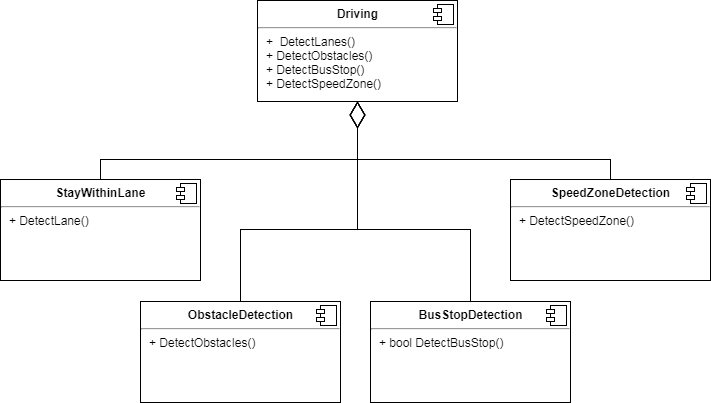
\includegraphics[width=\textwidth]{Images/Design/componentDiagram.png}
    \caption{Major components of functionality in the product; each component deals only with its own concerns}
    \label{fig:components}
\end{figure}
%Jeg er ikke overbevist om at ovenstående diagram er vildt vigtigt når vi nu alligevel har det nedenstående, dog giver det fint mening indtil videre

Note that the components refer not only to software, but also the physical design of the car. For instance, after we implement the driving component in software, we require a functioning LEGO-bus to test the software on. Only after this is done can we conclude whether the component works properly. Reason being that although the software logic might work as intended, incorrect sensor measurements, track/lane inconsistencies and similar need to be taken into account during programming, because otherwise the product might not work as expected.


\section{Software Architecture}
Because we are using nxtOSEK as our operating system for the bus \todo{has this been decided at this point in the report??, if not, then write it here}, we can program using either C or C++, see \ref{nxtOSEK} for more details. Because we can split the program cleanly into modular components as shown in the diagram \ref{fig:components}, we will program using the object-oriented programming paradigm in C++. 

Using the separated components as the baseline, we now create a class diagram that is less abstract than the component separation, which we will use as the software architecture of our model (the programming logic of the bus) implementation. Using this diagram, we will later create precise interfaces for all its classes. The dark blue boxes signify the physical sensors that the program will need to communicate with. 

The arrows on the figure signify function calls, e.g. if an arrow points from object A to B, it means that object A will call functions from object B. To better describe the concerns of each class on the diagram, we've written an example of one function call that might occur between the objects on each edge. This part isn't intended to be extremely precise, however, it helps communicate how we are planning to use object-oriented programming for information hiding and abstraction. See the diagram on \ref{fig:softwareArchitecture}

\begin{figure}[ht]
    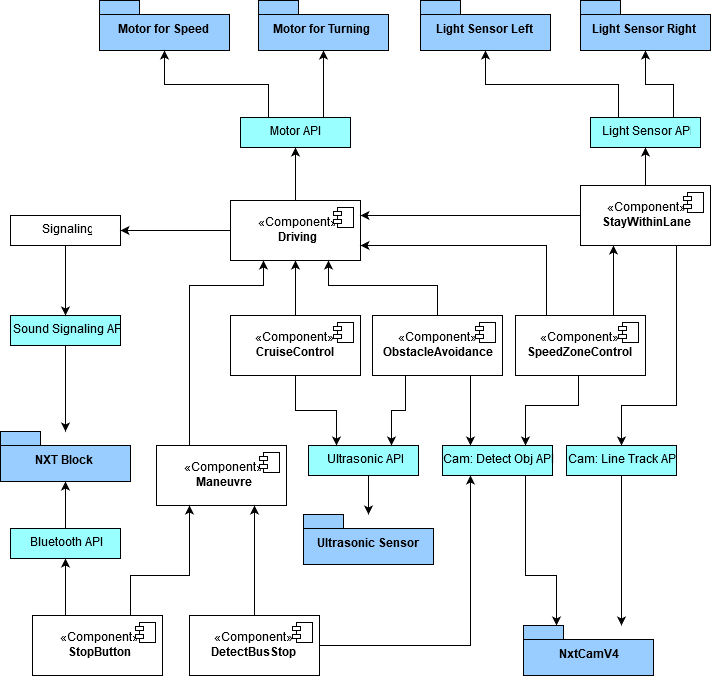
\includegraphics[width=\textwidth]{Images/Design/architectureClassDiagram.png}
    \caption{Class diagram of the program architecture of the model; function call examples are written on the edges}
    \label{fig:softwareArchitecture}
\end{figure}

The intent is that we use this diagram directly for our program architecture, so that each object on the diagram becomes a class in the implementation. The light blue coloured API-objects are also classes that we will create ourselves. The point with these is that they expose the useful functions that each sensor/actuator has, while also automatically filtering out incorrect measurements and calibrating the sensors.
%The figure above shows the implementation of our model, ie. the software of the bus that we write ourselves.

Do, however, note that the diagram is still a bit of a simplification. Specifically, the sensor API classes do not communicate directly with their corresponding sensors; instead they all query the NXT block, that gives access to different functions dependant on which sensors are connected. The diagram simply shows the model of the program, so we don't wish to directly deal with these sorts of implementation and low-level details. 

Something to note, which is not mentioned on the diagram, is that we have also planned to write a program separate from the system, which has the one job of sending messages via bluetooth to the NXT-block whenever we wish to illustrate that a passenger has clicked the stop-button. This is intended to work just like a stub-function would, and the rest of the program simply pretends that a real passenger clicked a button inside the bus.


\section{System Architecture}
As previously mentioned, there are many layers of abstraction in the program before one actually reaches the hardware level of the sensors. In this section, we will describe these layers, going from the high-level programming of the model, e.g. the architecture described on figure \ref{fig:softwareArchitecture}, down to the hardware specifics of the sensors themselves. 

The intend is, of course, that these software abstractions will not affect our model implementation, aside from the fact that we have to include some libraries to facilitate sensor communication (for instance "ecrobot\_interface.h" and similar). See figure \ref{fig:abstractionLayers} for the system architecture and its layers of abstraction. The dark blue object "Components" consists of all the software inside the components planned in the previous section \ref{fig:softwareArchitecture}. 

\begin{figure}[H]
    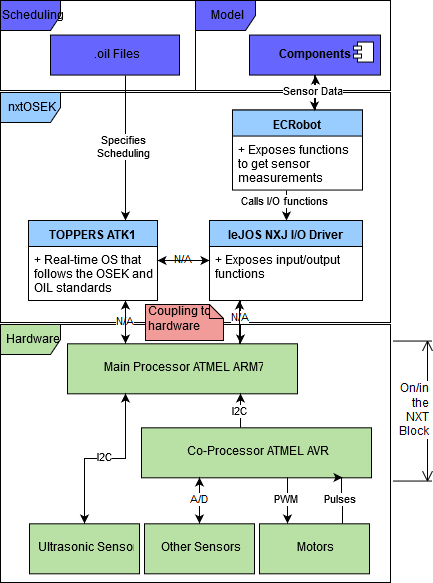
\includegraphics[width=\textwidth]{Images/Design/abstractionLayerDiagram.png}
    \caption{The system architecture of the product, going from high-level programming down to low-level hardware specifics}
    \label{fig:abstractionLayers}
\end{figure}

The note "Coupling to hardware" and the "N/A" edges exists because those are implementation details inside nxtOSEK, which we do not really have access to. In the hardware frame, the edges signify communication protocols such as PWM (pulse width modulation, as described in section \ref{analysisMotors}). 


\section{Interfaces}
In this section we specify interfaces for all objects in the software model, as seen in figure \ref{fig:softwareArchitecture}. This includes the API-objects, which are intended to abstract from hardware specific  information like the calibration of sensors and filtering out incorrect measurements from the raw data. 

\todo{Probably do this inside a draw.io diagram}

\subsection{API classes}
They all require a calibrate-method, which is called whenever the bus starts in order to ensure the sensors work as intended. 

\unsure{HOW DOES THIS WORK IN RELATION TO RTS and .oil files? How do we split all these functions into multiple tasks that can be scheduled using .oil files?}

\begin{description}
    \item [Motor]
    FindCentrum(); ???? Does this make sense for the motor for speed?
    SetRotation(int rpm, enum direction);
    
    \todo{Do I need an API for turning as well? or can I combine speed and turning in one?}
    
    The enum contains the choices: forwards and backwards. Rpm abbreviates rotations per minute.
    
    \item [LightSensor]
    \item [SoundSignaling]
    \item [Bluetooth]
    \item [Ultrasonic]
    \item [CamDetectObjects]
    \item [CamLineTracking]
\end{description}

\subsection{Other classes}
\subsection{API-objects}
\begin{description}
    \item [Signaling]
    void StartManeuvre(enum maneuvre);
    void EndManeuvre(enum maneuvre);
    enum CurrentManeuvre;
    
    The enum contains the choices: stopped, straight, turnLeft, turnRight, brake, reverse and emergency. 
\end{description}

\subsection{Component classes}
\begin{description}
    \item [Driving]
    void TurnDegrees(int targetDegrees, enum direction);
    void TurnDegrees(int degrees, enum inDirection);
    void SetSpeed(int targetKmHr, bool smooth);
    void IncreaseSpeed(int kmHr, bool smooth);
    void ReduceSpeed(int kmHr, bool smooth);
    void Stop(bool smooth);
    
    enum currentDirection;
    int currentTurn;
    int MaxSpeed;
    int CurrentSpeed;

    The enum contains the choices: left and right. The bool "smooth" decides whether the speed increase/decrease is gradual or not. 
    
    \item [Maneuvre]
    \item [StayWithinLane]
    \item [CruiseControl]
    \item [ObstacleAvoidance]
    \item [SpeedZoneControl]
    \item [StopButton]
    \item [DetectBusStop]
\end{description}

Additional to the software and system architecture, we will also design the bus itself along with the track that it needs to drive on. 
\todo{Write about the OSEK standard, And thereby also OIL, However, probably not in this chapter}

\section{Design of the track} \todo{This section needs to be checked for correctness.}

In order to validate that the requirements of the project are met. A track for the bus has to be made, and as such, tracks are designed with the goal of being able to complete the tasks, which are based on the requirements.

The track should have two lanes, as to mimic the pre-existing infrastructure, which usually has bidirectional roads. Furthermore the track should have bus stops that the vehicle can drive into, such that passengers can get on/off the bus.
The track should be designed to the scale of the bus, such that the turning rate of a corner should fit the maximum turning radius of the bus, and the width of the road should be designed after real danish roads based on the laws given by the danish road directorate \cite{roadRules}\cite{DriveingCurves}. As such the track needs be designed such that the bus has the needed space to turn around the corners without needing to reverse.

To help the sensors detect when to switch to a bus stop lane, the track should have special formed/coloured objects placed next to the bus stops, which sensor(s) can recognise. Furthermore if any people are standing at the bus stop to get onto the bus, they should be placed close to the bus stop sign.

To draw the track that the bus will drive on, black tape is used such that the sensors, which perform line tracking can more easily detect lines, and as such be able to stay within the lines. Black has been chosen over white, even though white is normally used to draw track lines. This is because white can be hard to detect due to light reflection. As such the tracks use black lines, as to to focus on a more complete bus implementation rather than focusing on tracking the lines.




% Selected Sensors:
%     \item[(4) Detecting Obstacles]
%    We intend to detect obstacles using a single sensor, which turns on whenever the bus is instructed to switch lanes, as to verify that no obstacles are found in the other lane. If this does not work, multiple sensors may be needed.